\documentclass[a4paper]{article}

\usepackage{mathtools} % математические формулы
\usepackage[T1,T2A]{fontenc} % кириллица
\usepackage[utf8]{inputenc} % кодировка шрифта кириллицы
\usepackage{indentfirst} %делать отступ в начале параграфа
\usepackage{enumerate} % нумерация списков
\usepackage{tabularx} % таблицы
\usepackage[english,russian]{babel} % вставка стороннего текста
\usepackage[12pt]{extsizes}
\usepackage{amsthm, amssymb, amsmath, amsfonts, nccmath, empheq}
\usepackage{color,colortbl} 
\usepackage[warn]{mathtext}
\usepackage{tocloft}  % для отточий в оглавлении
\linespread{1.5}
\usepackage{setspace} % для пробелов между линий
\usepackage{cmap}


\onehalfspacing
\usepackage{float}
\usepackage{graphicx}
\graphicspath{{pictures/}}
\DeclareGraphicsExtensions{.pdf,.png,.jpg}
\usepackage[left=25mm,right=25mm,
    top=2cm,bottom=30mm,bindingoffset=0cm]{geometry}
\renewcommand{\cftsecleader}{\cftdotfill{\cftdotsep}}

\usepackage{hyperref} % для гиперссылки на гитхаб

\author{Тырыкин Я. А. }
\date{March 2021}


\begin{document}
\begin{titlepage}
    \begin{center}
        \mbox{\normalsize{Санкт-Петербургский Политехнический Университет имени Петра Великого}}\\
        \normalsize{Институт Прикладной Математики и Механики}\\
        \large{\textbf{Кафедра "Прикладная Математика"}}
        
        \vfill
        
        \textbf{\Large{Отчет по лабораторной работе №4}}\\
        \textbf{\large{по дисциплине}}\\
        \textbf{\large"Математическая Статистика"}
        
        \vfill
        \raggedleft{Выполнил студент:}\\
        \raggedleft{Тырыкин Я. А.}\\
        \raggedleft{группа 3630102/80401}\\
        \raggedleft{Проверил:}\\
        \raggedleft{к.ф.-м.н., доцент}\\
        \raggedleft{Баженов А. Н.}\\
        
        % \normalsize{
        %     \begin{spacing}{0.5}
        %         \begin{tabular}{cc}
        %         Проверил: & \\\\ 
        %         к.ф.-м.н., доцент & Александр Николаевич Баженов \\\\
        %         Выполнил студент & \\\\
        %         группы 3630102/80401 & Ярослав Алексеевич Тырыкин \\\\
        %          \\\\
        %         \end{tabular}
        %     \end{spacing}
        % }\\
    
        
        \vfill
    
    \end{center}
    
    \begin{center} 
        Санкт-Петербург \\
        2021 
    \end{center}
\end{titlepage}
\newpage

% страница с оглавлением
% \renewcommand{\contentsname}{Оглавление} % можно поменять название оглавление
\begin{center}
    \tableofcontents
\end{center}
\setcounter{page}{2}
\newpage

% страница со сиском графиков
\begin{center}
    \listoffigures
\end{center}
\newpage

\section{Постановка задачи}
 Для 5 распределений:
 \begin{enumerate}
    \begin{item}
            Нормальное распределение \textit{N}(\normalsize{\textit{x}}, \normalsize{0}, \normalsize{1})
        \end{item}
        \begin{item}
            Распределение Коши \textit{C}(\normalsize{\textit{x}}, \normalsize{0}, \normalsize{1})
        \end{item}
        \begin{item}
            Распределение Лапласа \textit{L}(\normalsize{\textit{x}}, \normalsize{0}, \scriptsize{\dfrac{1}{\sqrt{2}}})
        \end{item} 
        \begin{item} 
            Распределение Пуассона \textit{P}(\normalsize{\textit{k}}, \normalsize{10})
        \end{item}
        \begin{item}
            Равномерное распределение \textit{U}(\normalsize{\textit{x}}, \normalsize{$-$\sqrt{3}}, \normalsize{\sqrt{3}})
        \end{item}
 \end{enumerate}
 Необходимо сгенерировать выборки размером 20, 60 и 100 элементов. Построить на них эмпирические функции распределения и ядерные оценки плотности распределения на отрезке $[-4; 4]$ для непрерывных распределений и на отрезке $[-6, 14]$ для распределения Пуассона.
 
\section{Теория}
    \subsection{Распределения}
    \begin{itemize}
        \begin{item}
            Нормальное распределение:
        \end{item}
        \begin{equation}\label{norm}
            \textit{N}(\normalsize{\textit{x}}, \normalsize{0}, \normalsize{1}) = \dfrac{1}{\sqrt{2\pi}}e^{\frac{{-x}^2}{2}}
        \end{equation}
        
        \begin{item}
            Распределение Коши:
        \end{item}
        \begin{equation}\label{cauch}
            \textit{C}(\normalsize{\textit{x}}, \normalsize{0}, \normalsize{1}) = \dfrac{1}{\pi}\dfrac{1}{x^2+1}
        \end{equation} 
        
        \begin{item}
            Распределение Лапласа:
        \end{item}
        \begin{equation}\label{lapl}
            \textit{L}(\normalsize{\textit{x}}, \normalsize{0}, \normalsize{\dfrac{1}{\sqrt{2}}}) = \normalsize{\dfrac{1}{\sqrt{2}}e^{-\sqrt{2}|x|}}
        \end{equation}
        
        \begin{item}
            Распределение Пуассона:
        \end{item}
        \begin{equation}\label{pois}
            \textit{P}(\normalsize{\textit{k}}, \normalsize{10}) = \dfrac{10^\textit{k}}{\textit{k}!}e^{-10}
        \end{equation}
        
        \begin{item}
            Равномерное распределение:
        \end{item}
        \begin{equation}\label{unif}
            \textit{U}(\normalsize{\textit{x}}, \normalsize{-\sqrt{3}}, \normalsize{\sqrt{3}}) = \begin{cases}
                                            \dfrac{1}{2\sqrt{3}} & \text{при $|\textit{x}|\leq\sqrt{3}$}\\
                                            0 & \text{при $|\textit{x}| > \sqrt{3}$}\\
                                       \end{cases}
        \end{equation}
    \end{itemize}
    \subsection{Эмпирическая функция распределения}
    
        \subsubsection{Статистический ряд}
        
            Статистическим рядом назывется последовательность различных элементов выборки $z_1, z_2, ..., z_k$, расположенных в возрастающем порядке  с указанием частот $n_1, n_2, ..., n_k$,  с которыми эти элементы содержатся в выборке. Статистический ряд обычно записывается в виде таблицы
            
            \begin{table}[H]
                \centering
                \begin{tabular}{|c|c|c|c|c|}
                    \hline
                     $z$ & $z_1$ & $z_2$ & $...$ & $z_k$ \\ \hline
                     $n$ & $n_1$ & $n_2$ & $...$ & $n_k$ \\ \hline
                \end{tabular}
                \caption{Статистический ряд}
                \label{tab:stat_series}
            \end{table}
            
        \subsubsection{Определение}
            Эмпирической (выборочной) функцией распределения (э. ф. р.) называется
относительная частота события $X < x$, полученная по данной выборке:

            \begin{equation} \label{emperic_function}
                F^*_n(x) = P^*(X < x)
            \end{equation}
            
        \subsubsection{Описание}
            Для получения относительной частоты $P^*(X < x)$  просуммируем в статистическом ряде, построенном по данной выборке, все частоты $n_i$, для которых элементы $z_i$, статистического ряда меньше $x$. Тогда $P^*(X < x) = \dfrac{1}{n}\sum\limits_{z_i < x}n_i$. Получаем
            
            \begin{equation}
                F^*(x) = \dfrac{1}{n}\sum\limits_{z_i < x}n_i
            \end{equation}
            
            $F^*(x) -$ функция распределения дискретной случайной величины $X^*$, заданной таблицей распределения:
            
            \begin{table}[H]
                \centering
                \begin{tabular}{|c|c|c|c|c|}
                \hline
                    $X^*$ & $z_1$ & $z_2$ & $...$ & $z_k$ \\ \hline
                    $P$ & $\dfrac{n_1}{n}$ & $\dfrac{n_2}{n}$ & $...$ & $\dfrac{n_k}{n}$ \\ \hline
                \end{tabular}
                \caption{Таблица распределения}
                \label{tab:distrib_table}
            \end{table}
            
            Эмпирическая функция распределения является оценкой, т. е. приближённым значением, генеральной функции распределения
            
            \begin{equation}
                F^*_n(x) \approx F_X(x)
            \end{equation}
            
    \subsection{Оценки плотности вероятности}
        
        \subsubsection{Определение}
            Оценкой плотности вероятности $f(x)$ называется функция $\widehat{f}(x)$, построенная на основе выборки, приближённо равная $f(x)$
            
            \begin{equation}
                \widehat{f}(x) \approx f(x)
            \end{equation}
        \subsubsection{Ядерные оценки}
            Представим оценку в виде суммы с числом слагаемых, равным объёму выборки:
            \begin{equation}
                \widehat{f}_n(x) = \dfrac{1}{nh_n} \sum\limits_{i=1}^n K(\dfrac{x - x_i}{h_n})
            \end{equation}
            Здесь функция $K(u)$ , называемая ядерной (ядром), непрерывна и является плотностью вероятности, $x_1, ... , x_n - $ элементы выборки, $\{h_n\} - $  любая последовательность положительных чисел, обладающая свойствами
            \begin{equation}
                h_n \underset{n \to \infty}{\longrightarrow} 0; \quad  nh_n \underset{n \to \infty}{\longrightarrow} \infty
            \end{equation}
            
            Такие оценки называются непрерывными ядерными.
            
            Гауссово (нормальное) ядро:
            
            \begin{equation} \label{Gauss_core}
                K(u) = \dfrac{1}{\sqrt{2\pi}}e^{-\dfrac{u^2}{2}}.
            \end{equation}
            
            Правило Сильвермана:
            
            \begin{equation} \label{Silverman_rule}
                h_n = 1.06\widehat{\sigma}n^{-1/5},
            \end{equation}
            
            где $\widehat{\sigma} - $ выборочное стандартное отклонение.

        \subsubsection{Оценка качества ядерных приближений}
        
            После получения результатов возникает необходимость оценить качество
ядерных приближений. Приведем в пример один из приемов количественных описаний сходства кривых - метод Фреше.

            Расстояние Фреше − это мера сходства кривых, принимающая во внимание число и порядок точек вдоль кривых. Расстояние названо по имени
французского математика Мориса Фреше. Метрика Фреше принимает во
внимание течение лвух кривых, посколько пары точек, расстояние между
которыми определяет расстояние Фреше, «пробегают» вдоль кривых. Расстояние Фреше между двумя кривыми − это не длина самого короткого
поводка, с котрым можно пройти все пути, а самый короткий, при котором
можно пройти этот путь.

            Определим кривую как непрерывное отображение $f : [a, b] \rightarrow V$, где $a, b \in R$ и $a \leq b$ и $(V, d) - $ метрическое пространство.  Даны две кривые $f : [a, b] \rightarrow V$ и $g : [a', b'] \rightarrow V$, их расстояние Фреше определено в виде:
            

\section{Модульная структура программы}
    Лабораторная работа выполнена с применением средств языка Python версии 3.7 в среде разработки PyCharm IDE (в частности, с применением встроенных методов библиотеки SciPy и MatPlotLib). Исходной код лабораторной работы находится по ссылке в приложении к отчёту.
\section{Результаты}
    \subsection{Эмпирическая функция распределения}
        \begin{figure}[H]
            \centering
            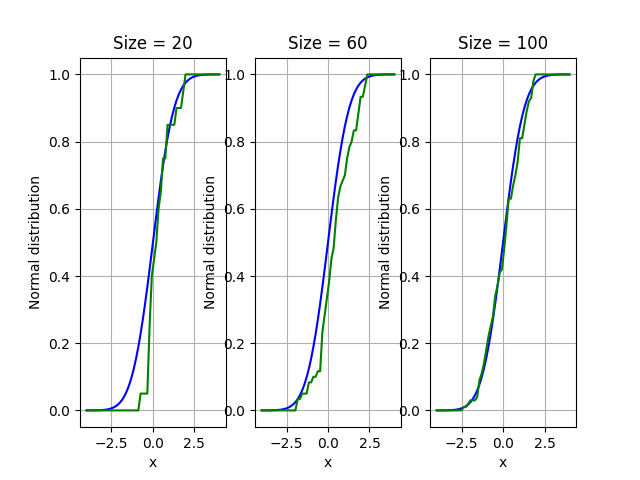
\includegraphics[scale = 0.4]{normal_distrib.png}
            \caption{Нормальное распределение \eqref{norm}}
            \label{fig:normal}
        \end{figure}
        
        \begin{figure}[H]
            \centering
            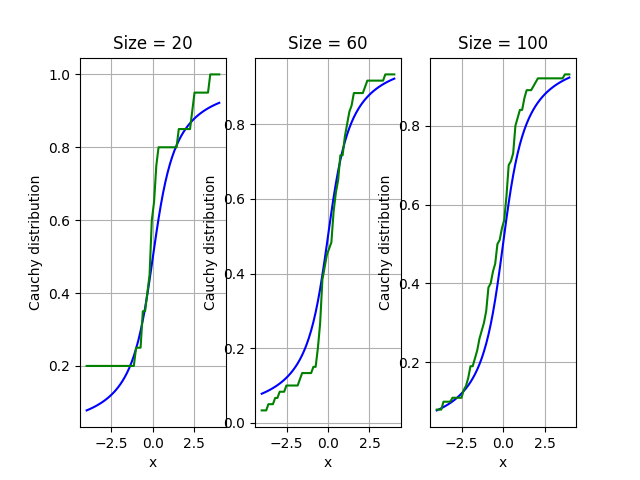
\includegraphics[scale = 0.4]{cauchy_distrib.png}
            \caption{Распределение Коши \eqref{cauch}}
            \label{fig:cauchy}
        \end{figure}
        
        \begin{figure}[H]
            \centering
            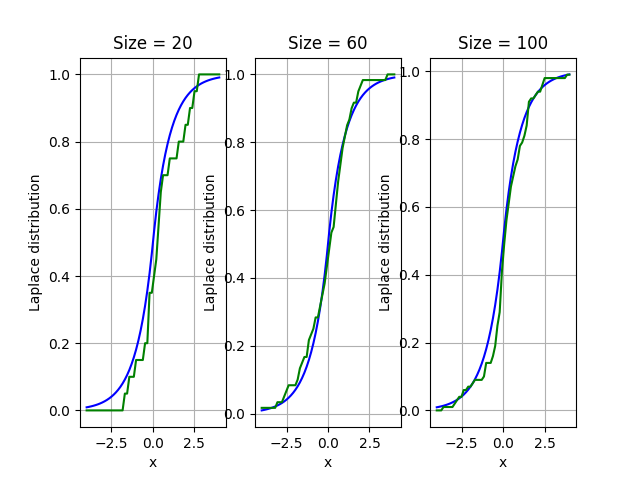
\includegraphics[scale = 0.4]{laplace_distrib.png}
            \caption{Распределение Лапласа \eqref{lapl}}
            \label{fig:laplace}
        \end{figure}
        
        \begin{figure}[H]
            \centering
            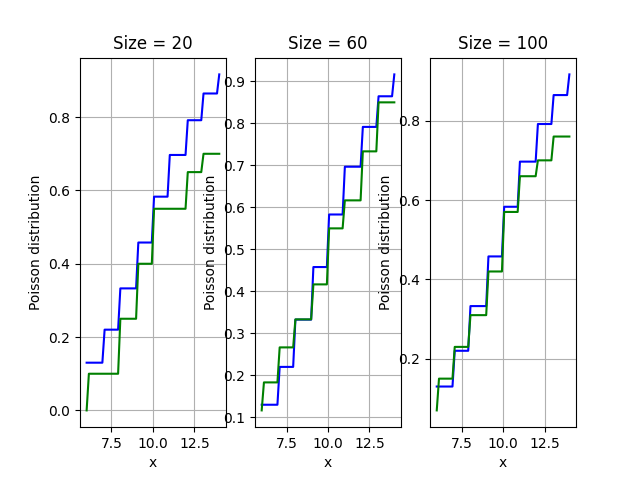
\includegraphics[scale = 0.4]{poisson_distrib.png}
            \caption{Распределение Пуассона \eqref{pois}}
            \label{fig:poisson}
        \end{figure}
        
        \begin{figure}[H]
            \centering
            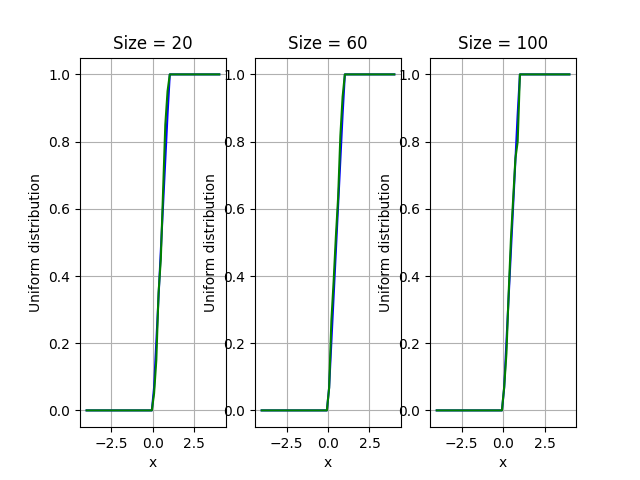
\includegraphics[scale = 0.4]{unifrom_distrib.png}
            \caption{Равномерное распределение \eqref{unif}}
            \label{fig:uniform}
        \end{figure}
        
    \subsection{Ядерные оценки плотности}
    
        \begin{figure}[H]
            \centering
            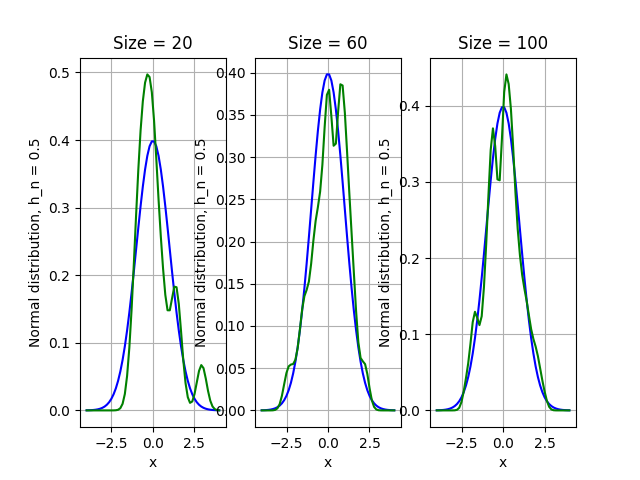
\includegraphics[scale = 0.4]{Normal distribution, h_n = 0.5.png}
            \caption{Нормальное распределение, $h_n = \frac{h_n}{2}$ \eqref{norm}}
            \label{fig:cauchy}
        \end{figure}
        
        \begin{figure}[H]
            \centering
            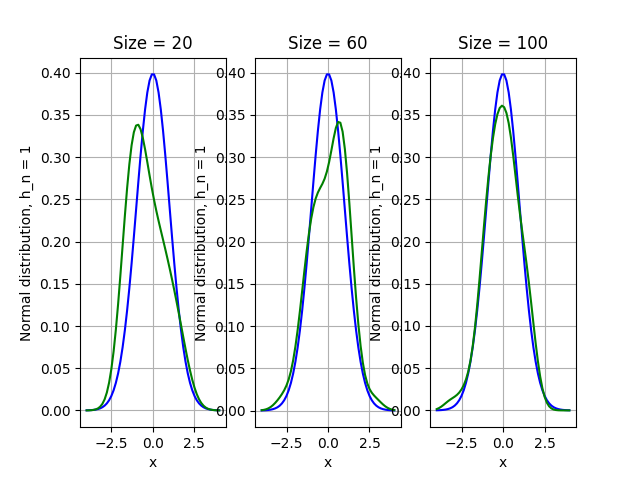
\includegraphics[scale = 0.4]{Normal distribution, h_n = 1.png}
            \caption{Нормальное распределение, $h_n = h_n$ \eqref{norm}}
            \label{fig:cauchy}
        \end{figure}
        
        \begin{figure}[H]
            \centering
            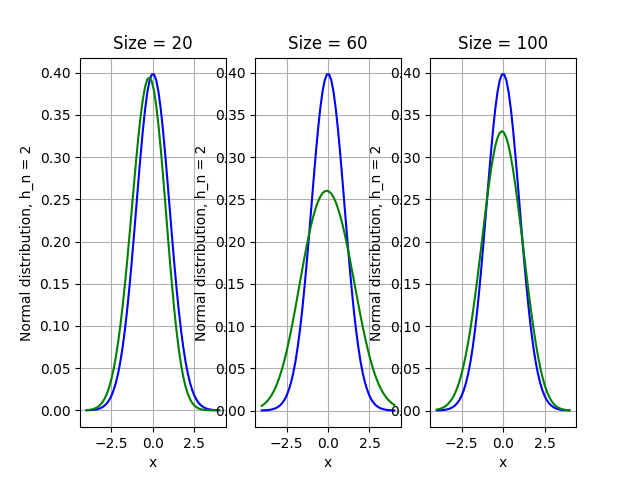
\includegraphics[scale = 0.4]{Normal distribution, h_n = 2.png}
            \caption{Нормальное распределение, $h_n = 2 h_n$ \eqref{norm}}
            \label{fig:cauchy}
        \end{figure}
        
        \begin{figure}[H]
            \centering
            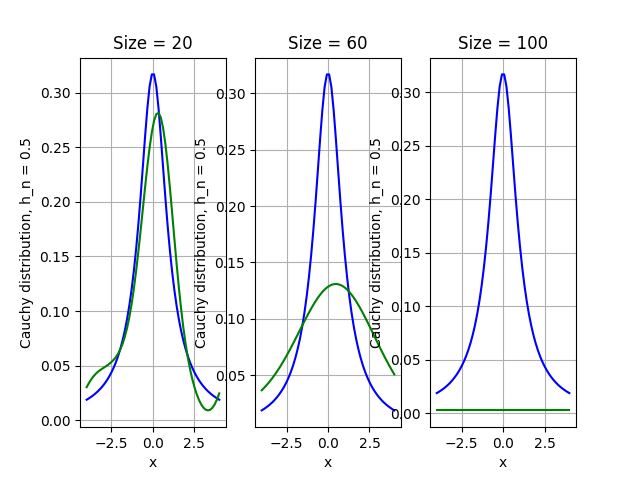
\includegraphics[scale = 0.4]{Cauchy distribution, h_n = 0.5.png}
            \caption{Распределение Коши $h_n = \frac{h_n}{2}$ \eqref{cauch}}
            \label{fig:cauchy}
        \end{figure}
        
        \begin{figure}[H]
            \centering
            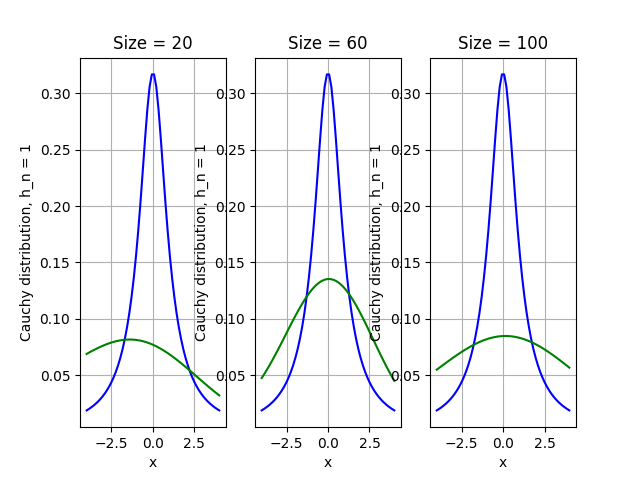
\includegraphics[scale = 0.4]{Cauchy distribution, h_n = 1.png}
            \caption{Распределение Коши $h_n = h_n$ \eqref{cauch}}
            \label{fig:cauchy}
        \end{figure}
        
        \begin{figure}[H]
            \centering
            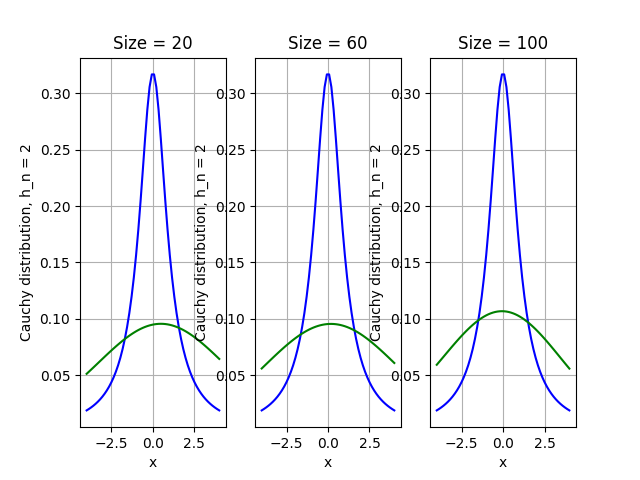
\includegraphics[scale = 0.4]{Cauchy distribution, h_n = 2.png}
            \caption{Распределение Коши $h_n = 2 h_n$ \eqref{cauch}}
            \label{fig:cauchy}
        \end{figure}
        
        \begin{figure}[H]
            \centering
            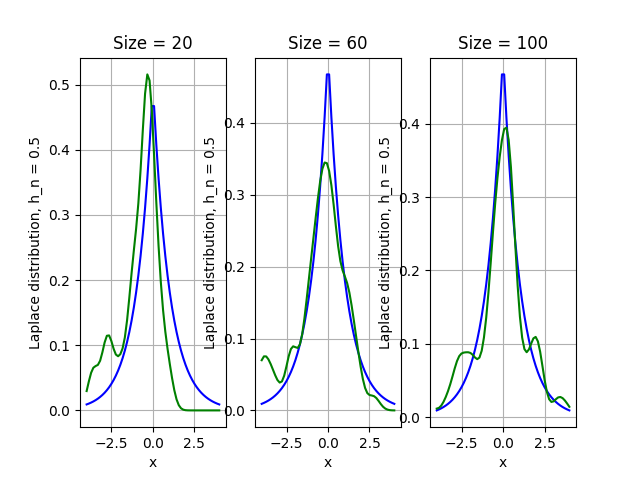
\includegraphics[scale = 0.4]{Laplace distribution, h_n = 0.5.png}
            \caption{Распределение Лапласа $h_n = \frac{h_n}{2}$ \eqref{lapl}}
            \label{fig:cauchy}
        \end{figure}
        
        \begin{figure}[H]
            \centering
            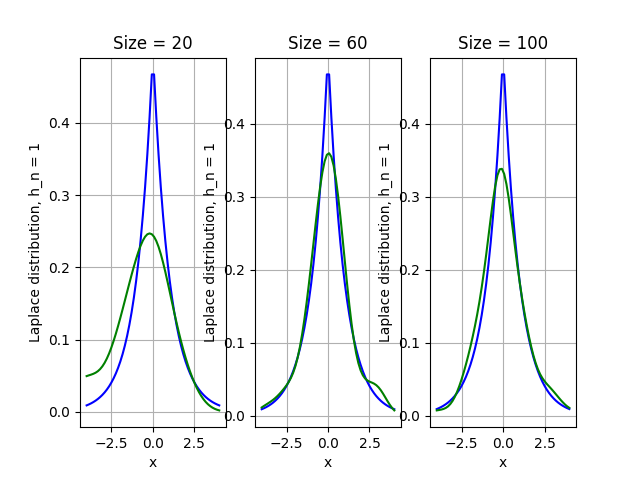
\includegraphics[scale = 0.4]{Laplace distribution, h_n = 1.png}
            \caption{Распределение Лапласа $h_n = h_n$ \eqref{lapl}}
            \label{fig:cauchy}
        \end{figure}
        
        \begin{figure}[H]
            \centering
            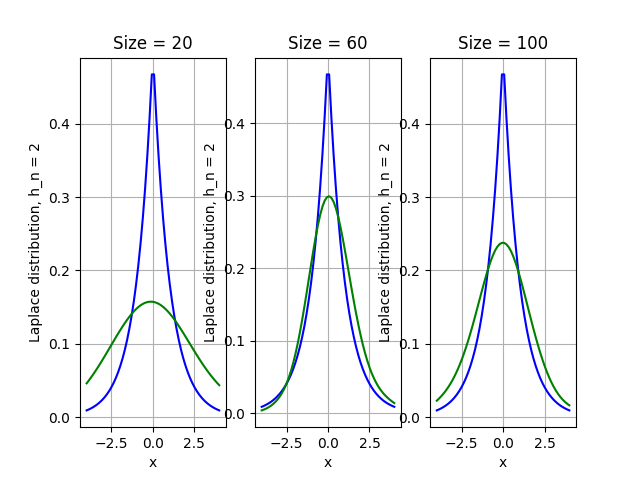
\includegraphics[scale = 0.4]{Laplace distribution, h_n = 2.png}
            \caption{Распределение Лапласа $h_n = 2 h_n$ \eqref{lapl}}
            \label{fig:cauchy}
        \end{figure}
        
        \begin{figure}[H]
            \centering
            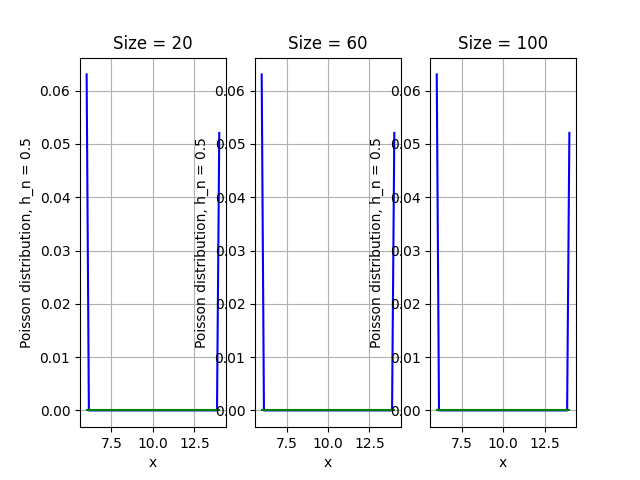
\includegraphics[scale = 0.4]{Poisson distribution, h_n = 0.5.png}
            \caption{Распределение Пуассона $h_n = \frac{h_n}{2}$ \eqref{pois}}
            \label{fig:cauchy}
        \end{figure}
        
        \begin{figure}[H]
            \centering
            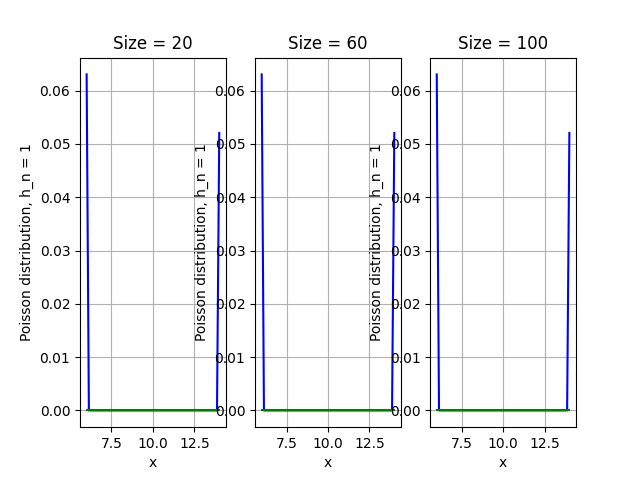
\includegraphics[scale = 0.4]{Poisson distribution, h_n = 1.png}
            \caption{Распределение Пуассона $h_n = h_n$ \eqref{pois}}
            \label{fig:cauchy}
        \end{figure}
        
        \begin{figure}[H]
            \centering
            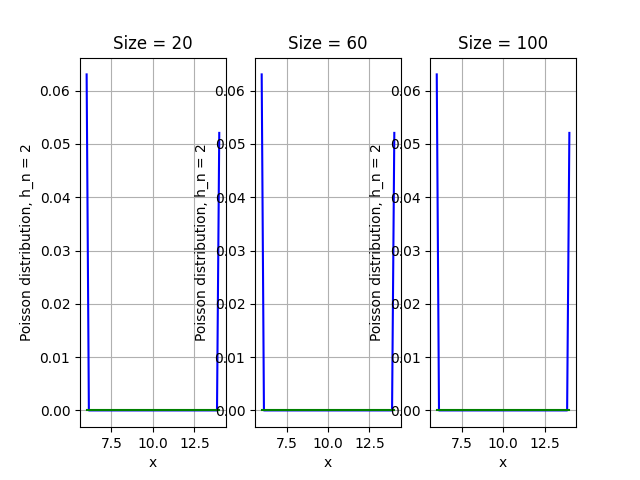
\includegraphics[scale = 0.4]{Poisson distribution, h_n = 2.png}
            \caption{Распределение Пуассона $h_n = 2 h_n$ \eqref{pois}}
            \label{fig:cauchy}
        \end{figure}
        
        \begin{figure}[H]
            \centering
            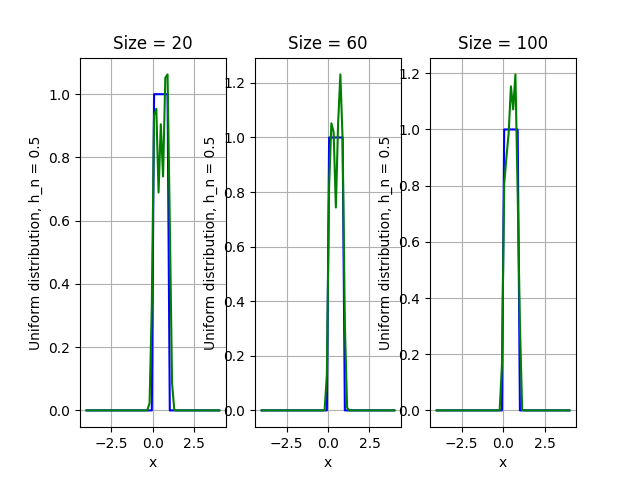
\includegraphics[scale = 0.4]{Uniform distribution, h_n = 0.5.png}
            \caption{Равномерное распределение $h_n = \frac{h_n}{2}$ \eqref{unif}}
            \label{fig:cauchy}
        \end{figure}
        
        \begin{figure}[H]
            \centering
            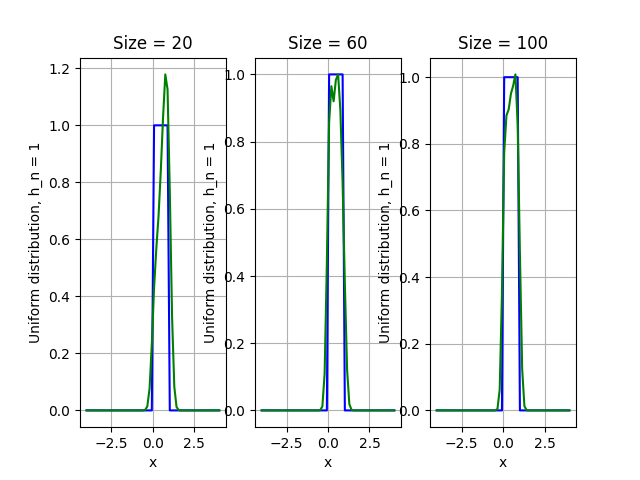
\includegraphics[scale = 0.4]{Uniform distribution, h_n = 1.png}
            \caption{Равномерное распределение $h_n = h_n$ \eqref{unif}}
            \label{fig:cauchy}
        \end{figure}
        
        \begin{figure}[H]
            \centering
            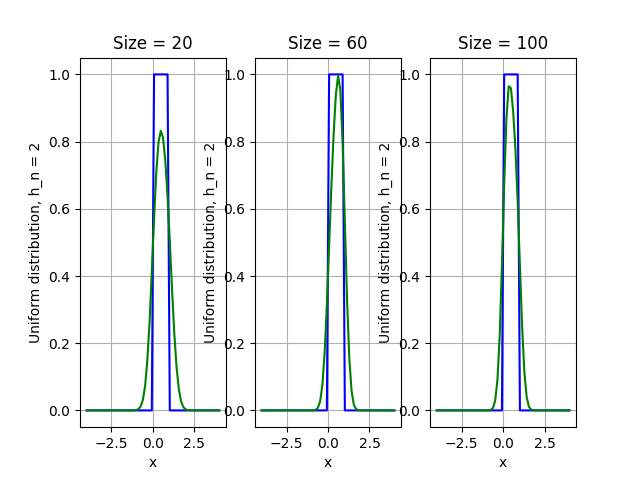
\includegraphics[scale = 0.4]{Uniform distribution, h_n = 2.png}
            \caption{Равномерное распределение $h_n = 2 h_n$ \eqref{unif}}
            \label{fig:cauchy}
        \end{figure}

    
\section{Обсуждение}
    \subsection{Эмпирическая функция и ядерные оценки плотности распределения}
        Можем наблюдать на иллюстрациях с э. ф. р., что ступенчатая эмпирическая функция распределения тем лучше приближает функцию распределения реальной выборки, чем мощнее эта выборка. Заметим так же, что для распределения Пуассона и равномерного распределения отклонение функций друг от друга наибольшее. //

        Рисунки, посвященные ядерным оценкам, иллюстрируют сближение ядерной оценки и функции плотности вероятности для всех $h$  с ростом размера выборки. Для распределения Пуассона наиболее ярко видно, как сглаживает отклонения увеличение параметра сглаживания $h$. \\
        
        В зависимости от особенностей распределений для их описания лучше подходят разные параметры $h$ В зависимости от особенностей распределений для их описания лучше подходят разные параметры $h = 2 h_n$, для распределения Лапласа - $h = h_n \ 2$, а для нормального распределения и распределения Коши - $h = h_n$. Такие значения дают вид ядерной оценки наиболее близкий к плотности, характерной данным распределениям. \\
        
        Также можно увидеть, что чем больше коэффициент при параметре сглаживания $\widehat{h_n}$  тем меньше изменений знака производной у аппроксимирующей функции, вплоть до того, что при $h = 2 h_n$ функция становится унимодальной на рассматриваемом промежутке. Также видно, что при $h = 2 h_n$ по полученным приближениям становится сложно сказать плотность вероятности какого распределения они должны повторять, так  как они очень похожи между собой. \\

\section{Ресурсы}
    \begin{spacing}{2.5}
        Код программы, реализующей отрисовку обозначенных распределений:
        
        \href{https://github.com/YaroslavAggressive/Mathematical-statistics-lab-works}{https://github.com/YaroslavAggressive/Mathematical-statistics-lab-works}
    \end{spacing}
\end{document}
